% Spice-weasel image enhancement manual

\documentclass[12pt, a4paper]{article}
%\usepackage[nofoot]{geometry}
\usepackage{graphicx}

\begin{document}

\title{Spice-Weasel photron image enhancement\\version 1.0}
\author{B.Dudson, UKAEA Fusion}
\date{July 12, 2006}

\maketitle

\tableofcontents

\section{MIT License}
Copyright (c) 2006 B.Dudson, UKAEA Fusion and Oxford University

Permission is hereby granted, free of charge, to any person obtaining
a copy of this software and associated documentation files (the "Software"),
to deal in the Software without restriction, including without limitation
the rights to use, copy, modify, merge, publish, distribute, sublicense,
and/or sell copies of the Software, and to permit persons to whom the Software
is furnished to do so, subject to the following conditions:

The above copyright notice and this permission notice shall be included in all
copies or substantial portions of the Software.

THE SOFTWARE IS PROVIDED "AS IS", WITHOUT WARRANTY OF ANY KIND, EXPRESS OR IMPLIED,
INCLUDING BUT NOT LIMITED TO THE WARRANTIES OF MERCHANTABILITY, FITNESS FOR A
PARTICULAR PURPOSE AND NONINFRINGEMENT. IN NO EVENT SHALL THE AUTHORS OR COPYRIGHT
HOLDERS BE LIABLE FOR ANY CLAIM, DAMAGES OR OTHER LIABILITY, WHETHER IN AN ACTION
OF CONTRACT, TORT OR OTHERWISE, ARISING FROM, OUT OF OR IN CONNECTION WITH THE
SOFTWARE OR THE USE OR OTHER DEALINGS IN THE SOFTWARE.

\section{Introduction}
In order to enhance interesting features present in photron fast-camera images,
 and to prepare stills for analysis or presentation, a code called ``Spice-Weasel''
(or just ``The Weasel'') has been developed. Anyone who watches far too many cartoons
will get the name. For everyone else, it's not important, and you'll just have to live
with it.

The code can read in either IPX videos as written by sergei shibaev's software
or a set of still images (in bitmap or PNG format). 
How the images are processed is controlled by a script whose syntax has been
designed to be (relatively) easy to write, to run efficiently, and to force
the result to be sensible. A feature of
the code is that it maintains a sliding window centred about a given frame-number,
allowing subtraction of several different ``background'' images.
The output is a set of images (again bitmap or PNG format) or an IPX video file.
Separate images can be used in presentations or converted to a video using software
such as VirtualDub. If both the
input and output are IPX files then frame times and header information are preserved,
although frame numbers will be different.

The weasel is designed to be as fast as i could make it: The amount of file reading
and writing is minimized and the code is multi-threaded (input, processing and output threads)
so that it can process images whilst waiting for file I/O to finish. Typically it will
process around 10 images per second on the fusion network machines, though this varies
depending on the processing steps and the size of the images.

This manual is divided into two initial sections describing how to use the code and the syntax
of the processing scripts, followed by a
technical section full of details most users won't need or want to know.
If you feel like modifying the code, this is the section for you.

To compile the code you will need libpthread, libpng (both standard on the fusion machines),
and the openjpeg10 library.

I hope people find this code useful, and if anyone finds a bug or writes improvements, please
let me know at ben.dudson@ukaea.org.uk. 

\section{Using Spice-Weasel}

To just run the weasel and see what happens, type

\begin{verbatim}
> spiceweasel 1000 1050 21 
\end{verbatim}

This will read in frames 1000 to 1050 inclusive from the default input file
(currently set to ``\texttt{\$MAST\_IMAGES/rbb/rbb015368.ipx}''). Using a window 21 frames wide,
i.e. 10 frames either side of a middle frame, the images will be processed using
the default script (see next section). This results in processed frames 1010 to 1040
which are output into the current directory as a set of PNG files named with the frame-number
as ``\texttt{processed\_1010.png}'' to ``\texttt{processed\_1040.png}''.

To set the input there is the ``\texttt{-i filename}'' option. For example, to read in another
nice photron file ``\texttt{\$MAST\_IMAGES/rbb/rbb015232.ipx}'' you could run

\begin{verbatim}
> spiceweasel 800 899 21 -i $MAST_IMAGES/rbb/rbb015232.ipx
\end{verbatim}

To save unnecessary typing and stave off RSI for a little while longer, 
if you want to read data for a given shot number from
the archive, there is the ``\texttt{-s shot}'' option. For example, to process the photron data for
shot 15236 from frame 200 to 400 with a window width of 21, run:

\begin{verbatim}
> spiceweasel 200 400 21 -s 15236
\end{verbatim}

In addition to reading IPX files, you may want to process a set of images from a different
source. To do this, the files should be in either bitmap (24-bit color) or compressed PNG
format. As long as the name of the file includes the frame number it doesn't matter. Instead
of giving the name of an IPX file with ``\texttt{-i}'', 
you specify a C printf format string for the filename. Another example is called for:

If you have a set of images in PNG format named ``\texttt{15232\_frame\_0500.png}'' to 
``\texttt{15232\_frame\_1200.png}''
in the directory ``\texttt{../data/}'' then to process these you would run:

\begin{verbatim}
> spiceweasel 500 1200 21 -i ../data/15232_frame_%04d.png
\end{verbatim}

The term ``\texttt{\%04d}'' will be replaced by the frame number. 
Just ``\texttt{\%d}'' will result in frame 500 becoming input file 
``\texttt{15232\_frame\_500.png}'', The number 4 specifies
4 digits, so ``\texttt{\%4d}'' would become ``\texttt{15232\_frame\_ 500.png}''
(note space before 500). The zero specifies zero padding of the number to produce
``\texttt{15232\_frame\_0500.png}''. For more info on C printf formatting, see
the manual page (\texttt{> man -S3 printf}).

The output settings work in the same way as the input except the option is
``\texttt{-o filename}''. To process shot 15100 and output to files of the form
``\texttt{15100\_frame\_00200.png}'' you would run something like:

\begin{verbatim}
> spiceweasel 100 300 21 -s 15100 -o 15100_frame_%05d.png 
\end{verbatim}

\noindent (Note 5 digits in frame number, hence \texttt{\%05d}). 

\section{Processing scripts}

The examples in the previous section used the default script to process the
input images. Called ``default.sps'',  this script is in the same directory as
the spiceweasel executable. 

Processing scripts currently have the extension \texttt{SPS} (for Spice-weasel Processing
Script) but this is optional. The scripts are not case-sensitive (\texttt{INPUT}
is the same frame as \texttt{input}), and a hash symbol comments out the rest of the line.
The syntax will be familiar to anyone who has written a Makefile
or coded in Haskell, consisting of blocks of code with the format:

\begin{verbatim}
<result image>: <input image(s)>
   <processing commands>
             .
             .
             .
\end{verbatim} 

\noindent Each of these blocks takes a set of input images, processes them and 
puts the final result into another image.
One of the blocks has to result in a final output image (called \texttt{output}).
The simplest possible script which would run is:

\begin{verbatim}
output: input
\end{verbatim}

\noindent which just copies the input frame (centre of the sliding window) to the output.
In addition to \texttt{input}, there are currently two other pre-defined frames:
\texttt{minimum} and \texttt{average}. These are the pixel-wise minimum and average over the
sliding window respectively, and can be used as background images because they smooth
over transient events like filaments.
To subtract the minimum background from the input frame, the processing command
\texttt{SUBTRACT} can be used:

\begin{verbatim}
output: input
  SUBTRACT minimum
\end{verbatim}

\noindent Because the difference between the input and the minimum images
is probably quite small (and hence produces a dim image),
the image could be amplified (in this case by a factor of 4):

\begin{verbatim}
output: input
  SUBTRACT minimum
  AMPLIFY 4.0
\end{verbatim}

Any number of extra processing steps could be applied to the output, but what if we want to process
the image in several different ways then combine them? Instead of writing the processed image
straight into the output, we can define a separate image called \texttt{difference}:

\begin{verbatim}
difference: input
  SUBTRACT minimum
  AMPLIFY 4.0
\end{verbatim}

\noindent This can then be combined with the original input image to produce the output:

\begin{verbatim}
output: input, difference
\end{verbatim}

\noindent If more than one image is put after the colon (separated by commas)
then these are put side-by-side (from left to right) to produce the image to be processed
by the following commands. The above example produces an image with the original on the left
and the background subtracted image \texttt{difference} on the right. Of course the combined
image can be processed further so to gamma correct the output, the script would be:

\begin{verbatim}
output: input, difference
  GAMMA 1.5

difference: input
  SUBTRACT minimum
  AMPLIFY 4.0
\end{verbatim}

The name of defined images can be any string except \texttt{input}, 
\texttt{minimum} and \texttt{average} since these are already defined. It can contain
any characters except space, tab, `\#', ':' and ','.
Defined frames can be used as inputs
for other images, or subtracted from each other. Obviously \texttt{output} cannot be used
as an input to anything. The order in which the frames are defined doesn't matter.
When the weasel first runs it will process the input script, producing errors if anything
is wrong. If the script has ``compiled'' correctly then the syntax is designed so that
it will always produce a sensible output without crashing (it may not look very good though!),
although i'm sure there are still many bugs to work out.
If you define frames but then don't use them then this will not slow down the processing; only
frames which are needed to produce \texttt{output} are calculated. The following example 
produces the original frame, the minimum background and the difference (gamma corrected). A
frame called \texttt{gamma\_frame} is defined, but is not needed for the output and so
isn't calculated.

\begin{verbatim}
output: input, minimum, difference

gamma_frame: input
  GAMMA 1.5

difference: input
  SUBTRACT minimum
  AMPLIFY 4.0
  GAMMA 2.0
\end{verbatim}

To specify a processing script, use the ``-p filename'' option. This will search:

\begin{enumerate}
  \item The local directory
  \item The directory pointed to by the environment variable \texttt{SPS\_PATH}
  \item The directory of the executable
\end{enumerate}
For example, say the spiceweasel executable is \texttt{/home/me/image\_proc/spiceweasel} and
you've set \texttt{SPS\_PATH = `/home/me/sps\_scripts/'}. Running spiceweasel from the home
directory \texttt{/home/me/} with:

\begin{verbatim}
> image_proc/spiceweasel 1000 1300 21 -s 15368 -p standard.sps
\end{verbatim}

\noindent will first look for \texttt{/home/me/standard.sps}, then \texttt{/home/me/sps\_scripts/standard.sps}
and finally \texttt{/home/me/image\_proc/standard.sps} and use the first it finds. If none are
found then the weasel will give up.

\subsection{Processing commands}
This section lists the processing commands which can be used in scripts and a brief description
of what they do. Some examples of the results are shown using frame 1020 from shot 15368.
When processing, pixels are converted into floating point values between 0.0 and 1.0, allowing
processing operations and the output precision to be set independently of input precision.

\subsubsection{SUBTRACT [subframe]}

This subtracts the specified frame \texttt{subframe} from the result frame.
\[
\texttt{frame} \rightarrow \texttt{frame} - \texttt{subframe}
\]

\subsubsection{NORMALIZE}

Amplifies and offsets an image so that the entire range is used.
\[
\texttt{frame}\rightarrow \left(\texttt{frame} - MIN(\texttt{frame})\right) / \left(MAX(\texttt{frame}) - MIN(\texttt{frame})\right)
\]

This will amplify each frame by a different amount but is good if you don't plan
on comparing magnitudes of different output frames.

\subsubsection{AMPLIFY [factor]}

Multiplies all frames by a constant value. 

\[
\texttt{frame}\rightarrow\texttt{frame}*factor
\]

\subsubsection{GAMMA [factor]}
Applies gamma correction a frame. If factor is greater than 1.0 then this will
enhance low-intensity pixels. Amplification is monotonic, so if one pixel is brighter than another
beforehand then it will be after gamma correction too.
\[
pixel \rightarrow pixel^{(1/\texttt{factor})}
\]

\begin{figure}[ht]
\centering
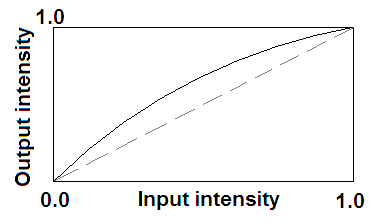
\includegraphics[width=0.5\textwidth]{gamma.png}
\caption{Gamma enhancement, $\texttt{factor} > 1.0$}
\end{figure}

\begin{figure}[ht]
\centering

\includegraphics[width=0.5\textwidth]{gamma_eg.png}
\caption{Gamma correction (2.0) of image 1020, shot 15368}
\end{figure}

\subsubsection{OFFSET [value]}
Adds a constant value to every pixel
\[
\texttt{frame}\rightarrow\texttt{frame} + value
\]

One use for this would be if you wanted to reverse the colors. The commands to do this
are:
\begin{verbatim}
AMPLIFY -1.0
OFFSET 1.0
\end{verbatim}
Another use is when subtracting frames except the minimum. This may result in negatives
which would normally be set to zero at the end. To display both positives and negatives
you could offset the frame to 0.5 (say).

\subsubsection{GAUSS\_BLUR [sigma]}
This blurs an image by averaging over a gaussian filter. \texttt{sigma} is the
standard deviation of the gaussian. The averaging is done over 3 sigma, so this can
result in a lot of processing.

\begin{figure}[ht]
\centering

\includegraphics[width=0.5\textwidth]{gaussblur_eg.png}
\caption{Gaussian blur (\texttt{sigma} = 3 pixels)}
\end{figure}

\subsubsection{DESPECKLE\_MEDIAN [radius]}
For evey pixel in the image this calculates the median value of the pixel and radius pixels
around it. For example, \texttt{DESPECKLE\_MEDIAN 1} calculates the median value of the pixels
in a 3x3 grid and puts the result in the central pixel.
This is very good at removing ``grainy'' noise
where some pixels are much brighter or dimmer than their neighbours.

\begin{figure}[ht]
\centering

\includegraphics[width=0.5\textwidth]{despeckle_eg.png}
\caption{Despeckling (radius 1)}
\end{figure}

\subsubsection{KUWAHARA [size]}

This is a non-linear smoothing filter also calculating median pixels, 
designed to preserve edges. Slower than median despeckling with (i think) no
real improvement. Try \texttt{KUWAHARA 1}.

%\begin{figure}[ht]
%\centering
%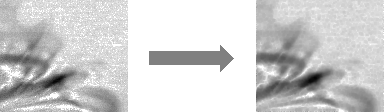
\includegraphics[width=0.5\textwidth]{kuwahara_eg.png}
%\caption{Kuwahara filter (size=1)}
%\end{figure}

\subsubsection{SHARPEN [k]}

This performs a simple sharpening of an image

\subsubsection{UNSHARP\_MASK [sigma] [amount]}

Performs unsharp masking on the image. A type of sharpening, this can work quite well. I've found
that \texttt{UNSHARP\_MASK 4.0 1.0} are good parameters. Like all sharpening, this will tend to
increase noise and so can be combined with a smoothing filter like despeckle.

\begin{figure}[ht]
\centering

\includegraphics[width=0.5\textwidth]{unsharp_eg.png}
\caption{Unsharp masking (4.0, 1.0)}
\end{figure}

Unsharp masking involves a lot of processing so can take a while
(due to gaussian blur step).
This command is actually a little superfluous because unsharp masking
can be done using the other commands:
\begin{verbatim}
usharp: input
  SUBTRACT blurmask

blurmask: input
  GAUSS_BLUR 4.0  # this is sigma
  SUBTRACT input
  AMPLIFY 0.5     # this is amount
\end{verbatim}

\noindent which takes \texttt{input} and puts an unsharp masked image in \texttt{usharp}.

\subsection{Useful script components}

In addition to performing basic unsharp masking, scripts can be written to perform
more complicated sharpening methods. A modification to the unsharp algorithm which
i've found gives quite good results when applied to either the original frame
or a differenced frame is:

\begin{verbatim}
usharp: input
  SUBTRACT blurmask

mask_input: input
  despeckle_median 1

blurmask: mask_input
  GAUSS_BLUR 4.0  # this is sigma
  SUBTRACT mask_input
  AMPLIFY 3.0     # this is amount
\end{verbatim}

The mask to apply (\texttt{blurmask}) is calculated from an image with the
noise removed (\texttt{mask\_input}), and then applied to the original image. 
This does not then amplify the noise but tends to sharpen features of the
image quite well.

\section{Technical details}

The spice-weasel code is written entirely in C. Parts of it are dependent on
POSIX features like pthreads, so it will only compile on UNIX-like systems.
It consists of four fairly separate parts: Input, processing, output and
syncronisation/book-keeping code which keeps the first three parts working. Parsing and running 
processing scripts is part of processing, but since it's the largest single bit
of source-code, it deserves a sub-section of its own.

\begin{figure}[ht]
\centering
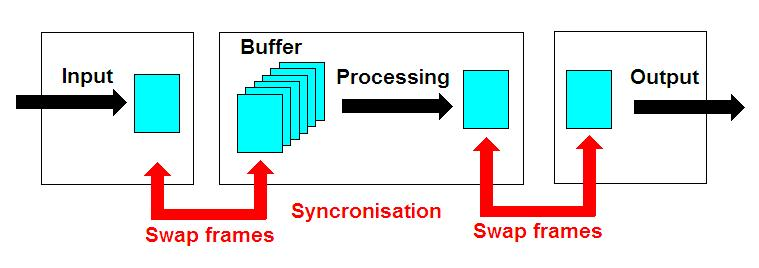
\includegraphics[width=0.9\textwidth]{blockdiagram.jpg}
\caption{Spice-Weasel block diagram}
\label{figblock}
\end{figure}

Figure \ref{figblock} shows how the parts of the code interact. The input thread
reads a single frame into memory (a TFrame structure), the processing thread maintains
a circular buffer of frames which are processed to produce an output frame and the output
thread writes a frame to disk. These tasks are done simultaneously to speed things up.
When a thread is finished it stops and waits for the others to finish too. Once all the 
threads have finished, the frame read by input is swapped with the oldest frame
in the circular buffer, the result from the last processing is swapped with
the frame in the output thread then the cycle begins again. When input reads the last
frame, it sets a flag in the TFrame structure which tells first the processing thread
then the output thread to stop.

Each image is stored in a structure called \texttt{TFrame}, defined in
\texttt{spiceweasel.h}:

\begin{verbatim}
typedef struct {
  int number;         /* Frame number */
  
  int width, height;  /* Width and height of frame (image) */
  int allocated;      /* Indicates whether data has been allocated */
  float **data;       /* A 2D array of pixel values */
  int last;           /* Flag indicating last frame */
}TFrame;
\end{verbatim}

\noindent Pixels are stored in columns as \texttt{data[column][row]}. This was to
make processing quicker, but at the expense of making reading and writing slightly
slower (since images are stored by rows).
The allocated flag is there because initially no pixel data is allocated. When a frame
is first used, memory is allocated and the flag is set. After this point the size
of a frame does not change. This is to minimize the amount of memory allocation
and freeing needed (again, speed was the deciding factor here).

\subsection{Input}

The input has to define three routines:
\begin{itemize}
\item \texttt{void read\_init()} Called once at the start of the program, this
should initialize any variables needed for reading. If reading an IPX file, this
code reads the IPX file header so that frames can be read quickly later.
\item \texttt{int read\_frame(int number, TFrame *frame)} This is called every
cycle and specifies which frame number to read and the location to put the data.
Returns 0 if successful.
\item \texttt{void read\_finish()} is called once at the end of the code and should
generally clean up. Currently just closes the input IPX file if used.
\end{itemize}

\subsection{Processing}

The processing code only has to supply two routines:
\begin{itemize}
\item \texttt{void process\_init()} sets up any temporary variables needed during
processing. For all but the simplest processing, intermediate frames are needed
and this routine marks them as unallocated so that the memory is allocated when
needed.
\item \texttt{int process\_frames(TFrame **framebuffer, int nframes, int centreframe,
TFrame *output)} Takes an array of frames (the frame buffer), the number of frames
in the buffer, the index of the frame in the centre of the window and the location
of the output frame.
\end{itemize}
A source file which supplies these is \texttt{process\_main.c} and is not
currently used, having been replaced by processing scripts (next sub-section).
Nevertheless it's still there and useful for testing etc. To compile a version
which uses this old code, just edit the \texttt{Makefile}, replacing
\texttt{run\_script.o} with \texttt{process\_main.o}. 

\subsection{Processing scripts}

This code takes a makefile-like processing script and produces a set of commands in a form
which can be quickly executed for each frame. This is done in three stages:
\begin{itemize}
\item {\bf Reading}: \texttt{parse\_newline()} reads the script, removing white-space
at the start of a line and comments and reducing all white-space to a single space. Letters are
capitalised. The first line containing useful characters is returned along with the line-number.
\item {\bf Processing}: \texttt{parse\_script()} first looks for target definitions which are
the only lines containing colons (after target name). If the line is a target then a new
target definition is begun (a \texttt{TTarget} structure), provided the name has not already been
defined. If the line is not a target then it is checked against a list of commands and, if valid,
added to the current target. All function names are converted into
ID numbers which are defined in \texttt{script.h}, for example ``AMPLIFY''
is changed to the constant \texttt{PROC\_AMPLIFY} (currently defined as 2).
The end result is an array of targets with a list of dependencies
and processing steps.
\item {\bf Resolving}: \texttt{resolve\_script()} is a recursive algorithm which starts by finding
the \texttt{output} target and its dependencies then the dependencies' dependencies and
so on. When a target is found which depends only on defined targets (such as \texttt{input})
it is assigned a temporary storage and the list of commands needed to create it are copied
to the final list. The result is a list of commands on temporary storage IDs instead of names
which results in the required \texttt{output}.
\end{itemize}

As an example, here's a script for unsharp masking the input:
\begin{verbatim}
# Modified unsharp masking with some despeckling

mask_input: input
    despeckle_median 1

blurmask: mask_input 
    GAUSS_blur 4.0 # this is sigma
    subtract mask_input
    # at this point this is the change
    # produced by bluring the image
    amplify 3.0  # this controls how much the image
                 # will be adjusted.

output: input
    # reverse change produced by bluring
    SUBTRACT blurmask
\end{verbatim}
The first (reading) stage will reduce this to:
\begin{verbatim}
MASK_INPUT:INPUT
DESPECKLE_MEDIAN 1
BLURMASK:MASK_INPUT 
GAUSS_BLUR 4.0
SUBTRACT MASK_INPUT
AMPLIFY 3.0
OUTPUT:INPUT
SUBTRACT BLURMASK
\end{verbatim}
The second (parsing) stage will find the three lines containing colons
and take these as definitions of \texttt{MASK\_INPUT}, \texttt{BLURMASK}
and \texttt{OUTPUT} targets. When an input is declared after a colon or used
as input for a command (such as \texttt{SUBTRACT MASK\_INPUT}), 
it is added to the dependency list for the target. 
This results in a tree-like structure shown in figure \ref{targetdeps} where
the dependencies are shown in red. 
\begin{figure}[ht]
\centering
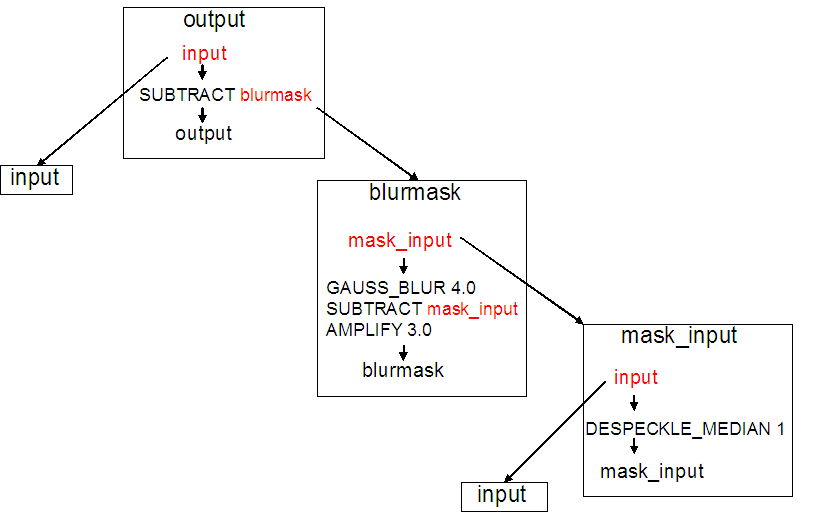
\includegraphics[width=0.9\textwidth]{script1.png}
\caption{Target dependencies for unsharp masking script}
\label{targetdeps}
\end{figure}

To resolve these dependencies and produce a list of commands to execute, the
function \texttt{resolve\_script()} calls \texttt{resolve\_script\_rec(char *name)},
passing \texttt{output} as the target name to resolve. This determines what targets
\texttt{output} depends on and calls \texttt{resolve\_script\_rec(char *name)} with
the names of those targets. The code works by travelling down the tree from \texttt{output},
following dependencies and then retracing its steps whilst copying the processing commands
needed and allocating temporary storage spaces.
For the current script, this produces the following steps:
\begin{enumerate}
\item First dependency of {output} is {input}. This is already defined so is set to
a special identifier \texttt{INPUT\_FRAME}.
\item Call \texttt{resolve\_script\_rec()} to resolve dependency \texttt{blurmask}
\item \texttt{blurmask} depends on \texttt{mask\_input} so call \texttt{resolve\_script\_rec()}.
\item \texttt{mask\_input} only depends on \texttt{input}, again set to \texttt{INPUT\_FRAME}.
\end{enumerate}
Now that \texttt{mask\_input} has all its dependencies, the processing steps are copied
into the final command list. Every function has an input and output frame and a number of
arguments (which may be frames too). In this case the function is \texttt{DESPECKLE\_MEDIAN},
and the input is set to \texttt{INPUT\_FRAME}. Every target must have its own storage space
which are given numbers, so \texttt{mask\_input} is set to storage space $\left<0\right>$ which is
the output of \texttt{DESPECKLE\_MEDIAN}. The command list is now:
\begin{verbatim}
Despeckle(INPUT, 1) => <0>
\end{verbatim}
At this point \texttt{mask\_input} has been assigned a storage space and so all dependencies of
\texttt{blurmask} have been resolved. The set of commands for \texttt{blurmask} are
are put at the end of the list.
The first command, \texttt{GAUSS\_BLUR} cannot have the same output as input since it operates
on several points, and so the next available storage space $\left<1\right>$ is used as output.
\texttt{SUBTRACT} and \texttt{AMPLIFY} can have the same input as output, 
and so both operate only on $\left<1\right>$. Finally, the end result is in $\left<1\right>$
and so \texttt{blurmask} is given ID 1. Now output has all its dependencies and so the same
thing happens, with the final result being given the special identifier \texttt{OUTPUT\_FRAME}.
\begin{verbatim}
Despeckle(INPUT, 1) => <0>
Gaussian blur(<0>, 4.000000) => <1>
<1> - <0> => <1>
<1> * 3.000000 => <1>
INPUT - <1> => OUTPUT
\end{verbatim}
In order to prevent circular dependencies, when a target is being resolved a flag
(\texttt{TTarget.resolving}) is set so that if the code tries to resolve the same
target twice without succeeding there must be a circular dependency and so an error
is reported.

The end result of processing a script is a \texttt{TCommands} structure:
\begin{verbatim}
typedef struct { /* Set of sequential commands for processing frames */
  int ntemp;         /* Number of intermediate frames needed */
  int minimum_frame; /* The ID of the minimum frame */
  int average_frame; /* ID of average frame */
  int nsteps;        /* Number of processing steps */
  TProcess *step;    /* List of processing steps */
}TCommands;
\end{verbatim}
If \texttt{minimum} or \texttt{average} are needed then their ID is set to be
a storage location i.e. $\ge 0$, otherwise they are not calculated. When
\texttt{process\_init()} is run, an array of \texttt{ntemp} frames is created
(called \texttt{tmp\_frame[]}) and frame IDs become indices into this array.
Each \texttt{TProcess} structure consists of
\begin{verbatim}
typedef struct {  /* Define a processing step */
  int method;       /* Which method to use */
  int nargs;        /* Number of arguments */
  int input;        /* Input frame */
  TProcArg *args;   /* Array of arguments */
  int result;       /* Result frame */
}TProcess;
\end{verbatim}
Because everything is specified as integers, a quick \texttt{switch} statement
can be used to select processing method. The function \texttt{get\_frame()} 
checks if a frame ID is is one of \texttt{INPUT\_FRAME} or \texttt{OUTPUT\_FRAME}
or an index into \texttt{tmp\_frame[]} and returns a pointer to the frame.
The arguments are stored as:
\begin{verbatim}
typedef struct { /* An argument to a processing step */
  char *name;   /* Name of frame (not used when processing) */
  float fval;
  int ival;
  int frame;    /* ID of frame */
}TProcArg;
\end{verbatim}
and so can be an integer, a float or a frame ID. The code which runs
the processing steps assumes that the script parsing code has worked
correctly and that the correct number and type of arguments are present
without performing any checks.

\subsubsection{Adding a processing command}

If you have a favourite image processing algorithm which i haven't included
and which can't be scripted then adding a new command may be worth it.

\begin{enumerate}
\item The first step is (obviously) to write the function to process the frames - see
the file \texttt{process\_frames.c} for the current set of functions. I strongly
recommend using the following code: 
\begin{verbatim}
  if(allocate_output(width, height, output)) {
    return(1);
  }
\end{verbatim}
where \texttt{output} is the output \texttt{TFrame*} pointer. This function checks
if the output frame has been allocated and if not then allocates memory. If it has,
the code checks that the sizes match and if not then returns nonzero. This ensures
that frame sizes are consistent and that memory is allocated once only. Other useful
functions are \texttt{shell\_sort()} and a set of routines for defining and applying
spatial filters to images which are used by \texttt{gauss\_blur()}.
Once you have written the function, put a prototype in \texttt{spiceweasel.h} with
the others.
\item Around line 25 in \texttt{script.h} there is a list of \texttt{\#define}
  statements like \texttt{\#define PROC\_KUWAHARA 6}. Add a new identifier for your function
  in the same way.
  If your function cannot have the same output as input then you need to add the identifier to the
  array \texttt{int proc\_noio[6]} before the last \texttt{PROC\_NULL}.
\item In function \texttt{parse\_script} in file \texttt{process\_script.c} starting around
  line 387 are a set of string comparisons like:
\begin{verbatim}
  }else if(strcmp(buffer, "AMPLIFY") == 0) {
    curproc->method = PROC_AMPLIFY;
    /* Should have one floating-point argument */
    if(nprocargs != 1) {
      printf("Error line %d: Amplify has one argument\n", linenr);
      return(1);
    }
    if(add_floatarg(curproc, procarg[0])) {
      printf("Error line %d: Argument to amplify is a floating point number\n", linenr);
      return(1);
    }
  }
\end{verbatim}
  Add a similar section (remember the string must be in capitals). The number of
  arguments passed is in \texttt{nprocargs} and the arguments are stored as an array
  of strings \texttt{procarg[]}.
  Set \texttt{curproc->method} to your function identifier defined in script.h. For each
  argument you can use the functions \texttt{add\_framearg}, \texttt{add\_floatarg}
  and \texttt{add\_intarg} to add a frame, float or integer argument respectively. These
  functions return non-zero in the event of an error and should be added in the order
  in which they appear in your function call.
\item Add a \texttt{case} statement for your function to \texttt{process\_frames()}
  in {run\_script.c} around line 137. This is a switch on function identifier
  (as defined in \texttt{script.h}). Already defined are \texttt{TFrame} pointers
  \texttt{in} and \texttt{out} for the input and output frames. 
  \texttt{proc->args[]} is an array of \texttt{TProcArg} structures for the
  arguments with \texttt{ival} and \texttt{fval} elements for integer and floating point
  values respectively. To pass a pointer to a frame, use the macro
  \texttt{GETFRAME(proc->args[i].frame)}.
\item (optional) Add your function to \texttt{dummy\_script()} in
  \texttt{process\_script.c}. This prints out the processing steps to be performed
  at the start of the program but does no actual processing. 
\end{enumerate}

\subsection{Output}

Like the input, the output code defines three routines:
\begin{itemize}
\item \texttt{void write\_init()}
\item \texttt{int write\_frame(TFrame *frame)}
\item \texttt{void write\_finish()}
\end{itemize}

\subsection{Syncronisation code}

\end{document}
